\usepackage{gensymb}

\begin{document}
%
% paper title
% can use linebreaks \\ within to get better formatting as desired
\title{Model Driven Development in Power Electronics}


% author names and affiliations
% use a multiple column layout for up to three different
% affiliations
%\author{
%\IEEEauthorblockN{David Kiss}
%\IEEEauthorblockA{School of Electrical and\\Computer Engineering\\
%Georgia Institute of Technology\\
%Atlanta, Georgia 30332--0250\\
%Email: http://www.michaelshell.org/contact.html}
%\and
%\IEEEauthorblockN{Homer Simpson}
%\IEEEauthorblockA{Twentieth Century Fox\\
%Springfield, USA\\
%Email: homer@thesimpsons.com}
%\and
%\IEEEauthorblockN{James Kirk\\ and Montgomery Scott}
%\IEEEauthorblockA{Starfleet Academy\\
%San Francisco, California 96678-2391\\
%Telephone: (800) 555--1212\\
%Fax: (888) 555--1212}}

% conference papers do not typically use \thanks and this command
% is locked out in conference mode. If really needed, such as for
% the acknowledgment of grants, issue a \IEEEoverridecommandlockouts
% after \documentclass

% for over three affiliations, or if they all won't fit within the width
% of the page, use this alternative format:
% 
\author{\IEEEauthorblockN{David Kiss\IEEEauthorrefmark{1},
Adam Halmos\IEEEauthorrefmark{1},
Gergely Kalman\IEEEauthorrefmark{1}, 
Istvan Varjasi dr.\IEEEauthorrefmark{2} and
Zoltan Suto dr.\IEEEauthorrefmark{2}}
\IEEEauthorblockA{\IEEEauthorrefmark{2}Budapest University of Technology and Economics\\
Deparment of Automatization and Applied Informatics}
\IEEEauthorblockA{\IEEEauthorrefmark{1}Hyundai Technologies Center Hungary Ltd., Budapest, Hungary\\
Email: dkiss@h-tec.hu; ahalmos@h-tec.hu; gkalman@h-tec.hu}
}



% use for special paper notices
%\IEEEspecialpapernotice{(Invited Paper)}


% make the title area
\maketitle


\begin{abstract}
%\boldmath
Nowadays power converters are gaining more and more importance due to the increasing demand of energy efficient solutions in industrial applications, renewable energy sources and electrical transportation. To meet this new demand, development cycles must be shortened, without compromising the quality of the control software. This goal can be achieved with model driven development, and it also can make the process more agile. In the presented method, we are using MATLAB Simulink to implement the control related software components. These software modules, such as control loops and state machines can be functionally tested in the Simulink environment, with much better observability than the real embedded software. The embedded code is generated from these models. The embedded code only contains the framework, which is providing a interface between the model and the control peripherals and the real time operating system. In this paper we are discussing the process in detail on a frequency converter firmware as example.
\end{abstract}
% IEEEtran.cls defaults to using nonbold math in the Abstract.
% This preserves the distinction between vectors and scalars. However,
% if the journal you are submitting to favors bold math in the abstract,
% then you can use LaTeX's standard command \boldmath at the very start
% of the abstract to achieve this. Many IEEE journals frown on math
% in the abstract anyway.

% Note that keywords are not normally used for peerreview papers.
\begin{IEEEkeywords}
IYCE, Power Electronics, MATLAB, Simulink, Motor Control, VFD, Model Driven Development
\end{IEEEkeywords}


% For peer review papers, you can put extra information on the cover
% page as needed:
% \ifCLASSOPTIONpeerreview
% \begin{center} \bfseries EDICS Category: 3-BBND \end{center}
% \fi
%
% For peerreview papers, this IEEEtran command inserts a page break and
% creates the second title. It will be ignored for other modes.
\IEEEpeerreviewmaketitle


\section{Introduction}
A modern VFD system must comply to many customer requiroments. There are also many industrial standard such as power factor regulations and EMC limitations wich are needed to control by software. The computation power of the embeddedd microcontrollers are capeble to achive this kind of sophistication, but the this power needed to be utilized by the programmer efficiently. The development cycles also getting shorter and shorter to met the constantly changing market demand. Therfore a modular, reusable and scalable control software need to be implemented.

One of the ways of this new way of thinking about software development is model-driven or model-based development. This means we are using graphical diagrams to describe the desired functionality instead of lines of program code. In power electronics this kind of abstraction can seem contradictionary, becouse  of the strict timing constraints, but as this paper will show, with the correct methodes high level problem solving and low level IO handling can go hand in hand. There are even many benefits of model-based desing due to the implemented control loops and state machines, wich can be easily viusalised and simulated with the proper software tool.

Modern software tools such as MATLAB and Simulink are very well suited to this task. The Embedded Coder toolbox generates the C code, wich can be complied in the embedded processor. Becouse the model is developped in Simulink, the behaviour of the implelemnted control algorythms can be tested immediatly, on the PC. When the simulations sows the desired results, the C code can be generated. This generated C code is 

In the II. chapter we are going to discuss the embedded framework, wich provides the connection between the Simulink model and the real microcontroller outputs and inputs. The III. chapter will present a short insight in the Simulink model, and present the challanges you can face during the development. The IV. chapter will provide a case study about the whole method. The example will be a IGBT thermal model. We will compare the simulated data and the measured tempereatures.


\section{Embedded Framework}

The embedded framework provides connection between the generated code and the hardware peripherials. All the hardware dependent code is written in native C language. The scheduling of the generated code is made by an embedded operation system and hardware interrupts (timers, analog-digital converters, etc.). In this case all the generated code is hardware independent and reusable. The model connects to the embedded code thrugh interfaces. These interfaces are represented as Buses in Simulink and structs in C. The input structs contain the parameters and the and the measured inputs, the output interfaces give signals for the embedded operation framework (start stop signals etc.) and give the calculated duty cycles and the switching frequency. 
On every PWM timer cycle timer interrupt is given. The timer pheripherial gives an interrupt to AD converters a new set of measurements available (Three phase currents and the DC voltage). The values which change slower then the switching period are measured in the main task. The measured AD values calculated to values in SI units. The outputs of the model are also in normalized number. In this case the connection between the embedded code and the model is also platform independent. Example the structure of the measured input values:

\begin{lstlisting}
typedef struct \{ \\
  real32_T VxMeasured; \\
  real32_T VyMeasured; \\
  real32_T Vdc; \\
  real32_T Ia; \\
  real32_T Ib; \\
  real32_T Ic; \\
  real32_T Ta; \\
  real32_T Tb; \\
  real32_T Tc; \\
  real32_T Tinner; \\
  real32_T Tbrake; \\
  real32_T V5Sto1Meas; \\
  real32_T V5Sto2Meas; \\
  real32_T V15Meas; \\
  real32_T FANSpeed1; \\
  real32_T FANSpeed2; \\
\} MeasurementIn;

\end{lstlisting}

All the measured inputs are 32 bit floating point numbers, the values start with V are voltages the values start with I are currents and the values start with T are temperatures.

\subsection{Scheduling the tasks}
For scheduling an embedded operation system is used. In this particular project the Keil RTX operation system is used. This Keil RTX has all the necessary tools for this project task priority levels timer functions and os signals. As it was mentioned above the PWM timer schedules the measurement of the DC voltage and the phase currents. After the measurements completed and the values calculated to their normalized values the motor control fast task is called. This task calculates the pwm duty cycle from the input and the given setpoint and checks whether the measured values exceed the predefined limits. 
There is a lower priority task which scheduled by the os timer. This task provides operation framework and the compute intensive functions are also placed there. The structure of the Simulink model is described on the following chapter.



\section{Simulink Model}
To be able to make offline measurements ans simulations the whole system is modeled with the excitations the inverter and the plant. Therefore the offline simulations can be done in Matlab Simulink enviroment and results can be compared to real life measurements. Testing is also important part of this model based developement. Thatswhy unit test enviroment built for every functional part of the of the inverter. To be able to test every part separeted, test enviroments has been made for them. These functions has the same input and output ports like the main model and the functionality models connect eachother through them. In Simulink the test excitations are given through these inputs and a behaviour is monitored through the outputs of these subsystem.  On the following chapters a case study is described about the IGBT thermal model.
To be able to 

Közös interfészek
globális változók
reference subsystem
nagy teszt kis teszt

\section{Case Study: IGBT Thermal model}

\subsection{The function of the Thermal model}
The semiconductor switches maximum allowable temperature is limited. The absolute maximum junction temperature of silicium based devices  are $175\ \degree{}C$ degrees. It is advisable to take the advantage of this temperature to keep the volume/power ratio as low as possible. The thermometer placed in the heat sink or in the semiconductor case does not provide suefficient information about the actual junction temperature of the semiconductor elements. However semiconductor junction temperatures can be calculated knowing the thermal model between the thermometer and the semiconductor junction. The model parameters and the model type are described in the datasheets. The junction temperatures can be calculated from the diode and transistor losses.

\subsection{The offline model}
The IGBT junction temperature calculation module structure is based on the principles laid down the full model description. The thermal model calculates the three phase bridge and the brake IGBT temperatures. The calculation method can be generalized, it is the same in every phase legs. The brake transistor is basically a truncated phase containing only the bottom transistors and freewheeling diode. With the following assumptions the temperute calculation can be simplified to only one transistor loss calculation:

\begin{itemize}
    \item The inductance of the brake resistor is neglectable, therfore the current carried by the diode can be also neglected
    \item The switching loss of the diode can be also neglected, becouse the high power is carried by the IGBTs
    \item With the two assumptions above, we can also use the PWM controls signals directly in the loss calculation.
\end{itemize}

Due to the above considerations phase IGBT temperature and brake IGBT temperature library blocks created as building block elements. The library block interface is containing the input signals, the output signals and the parameter bus as discussed in the model description part.
The input bus is containing the current, the DC voltage and the duty cycle of the respective phase, switching frequency, case temperature. The parameter bus is containing the IGBT and the diode electrical and thermal parameters. The output bus is containing the IGBT and diode losses and temperatures. The parameters are calculated with a MATLAB script which contains the values from the datasheet and values derived from these parameters.

The library blocks can be separeted to three main parts:
\begin{itemize}
    \item Duty cycle calculation of the individual semiconductor (diode, IGBT) elements
    \item Switching and conduction loss calculations for each element.
    \item Temperature calculation from power losses using a three tie constant thermal model (Foster network or PI). 
\end{itemize}
Duty cycle calculation of the individual semiconductor (diode, IGBT) elements
Switching and conduction loss calculations for each element.
Temperature calculation from power losses using a three tie constant thermal model (Foster network or PI). 

The three phase half-bridge IGBTs and brake IGBT temperature calculation is integrated in the model. This model can be easily simulated in the test environment and in the integrated model as a referenced model.

\subsection{Offline test evironment}

The test harness structure is the following: on the left side are the parameters and excitations. These blocks connected with the thermal model placed in the middle with the buses used in the integrated model. Output is on the right side. A model block created to calcalutethe one period average values of the output. The average values used for comparison with Semisel calculator.

We can define the desired setpoint in the simulation environment. The simulink model source parameters are calculated with script. (Input parameters: DC voltage, phase current, $cos\phi{}$, switching frequency, heat sink temperature). The Simulink model generates the excitation signals during the simulation.

The Semisel calculator program is used for validating the calculated junction temperature. The Semisel software calculates the average temperature and the maximum temperature values of the selected device. Setting the same setpoint in the calculator program and in the simulation we expect the same result. The  semisel calculator doesn’t give information about the temperature vs time function, only shows the maximum temperatures. Because the junction temperatures are used for absolute temperature protections, comparing the simulated and calculated maximum temperature values is fullfilling our reuirements. The temperature should differ the direction of safety so the temperature values are considered to be acceptable if the difference of the simulated and calculated temperatures is in the 0.. +5 range.

After the successful offline simulation, C code is generated from the integrated model which was tested in the real inverter.
The case, junction temperatures, phase currents was recorded in different setpoints on a drive testbench. The temperature vs. time function was simulated in Sumilink, then the simulated and measured junction temperatures were  plotted in a coordinate system, which was synchronized with the corresponding phase currents. The results can be seen in the figure.

\begin{figure*}[!h]
\centering
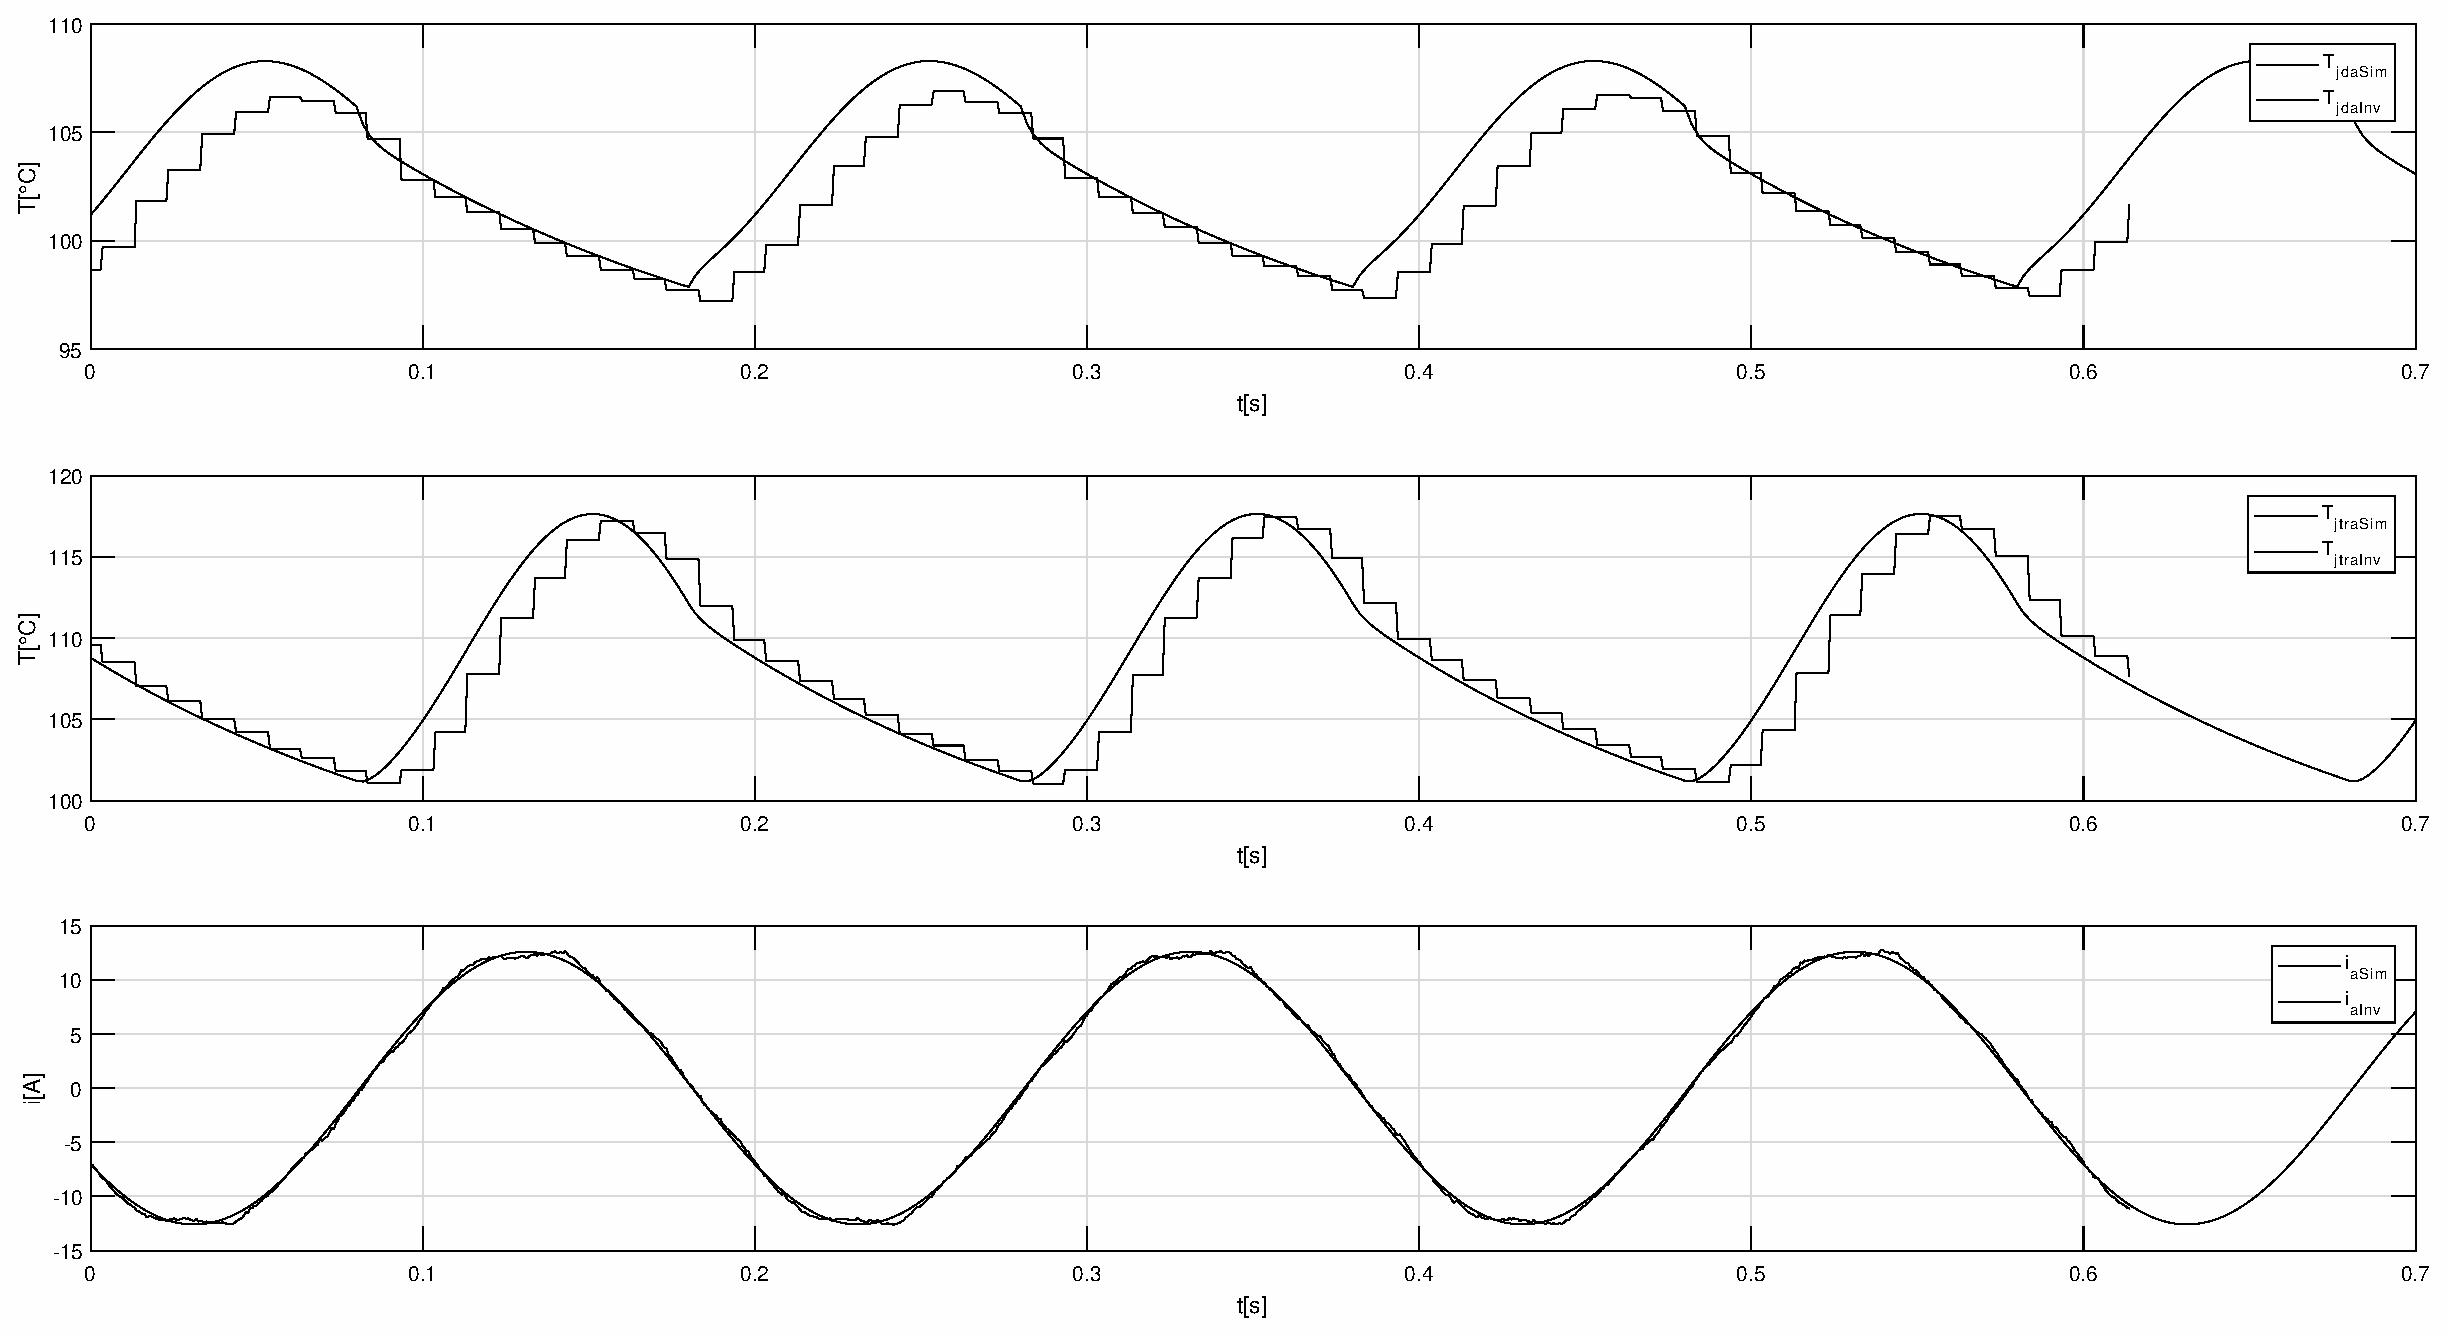
\includegraphics[width=0.8\textwidth]{figures/homerseklet}
% where an .eps filename suffix will be assumed under latex, 
% and a .pdf suffix will be assumed for pdflatex; or what has been declared
% via \DeclareGraphicsExtensions.
\caption{Simulation Results}
\label{fig_sim}
\end{figure*}

% needed in second column of first page if using \IEEEpubid
%\IEEEpubidadjcol

% An example of a floating figure using the graphicx package.
% Note that \label must occur AFTER (or within) \caption.
% For figures, \caption should occur after the \includegraphics.
% Note that IEEEtran v1.7 and later has special internal code that
% is designed to preserve the operation of \label within \caption
% even when the captionsoff option is in effect. However, because
% of issues like this, it may be the safest practice to put all your
% \label just after \caption rather than within \caption{}.
%
% Reminder: the "draftcls" or "draftclsnofoot", not "draft", class
% option should be used if it is desired that the figures are to be
% displayed while in draft mode.
%
%\begin{figure}[!t]
%\centering
%\includegraphics[width=2.5in]{myfigure}
% where an .eps filename suffix will be assumed under latex, 
% and a .pdf suffix will be assumed for pdflatex; or what has been declared
% via \DeclareGraphicsExtensions.
%\caption{Simulation Results}
%\label{fig_sim}
%\end{figure}

% Note that IEEE typically puts floats only at the top, even when this
% results in a large percentage of a column being occupied by floats.


% An example of a double column floating figure using two subfigures.
% (The subfig.sty package must be loaded for this to work.)
% The subfigure \label commands are set within each subfloat command, the
% \label for the overall figure must come after \caption.
% \hfil must be used as a separator to get equal spacing.
% The subfigure.sty package works much the same way, except \subfigure is
% used instead of \subfloat.
%
%\begin{figure*}[!t]
%\centerline{\subfloat[Case I]\includegraphics[width=2.5in]{subfigcase1}%
%\label{fig_first_case}}
%\hfil
%\subfloat[Case II]{\includegraphics[width=2.5in]{subfigcase2}%
%\label{fig_second_case}}}
%\caption{Simulation results}
%\label{fig_sim}
%\end{figure*}
%
% Note that often IEEE papers with subfigures do not employ subfigure
% captions (using the optional argument to \subfloat), but instead will
% reference/describe all of them (a), (b), etc., within the main caption.


% An example of a floating table. Note that, for IEEE style tables, the 
% \caption command should come BEFORE the table. Table text will default to
% \footnotesize as IEEE normally uses this smaller font for tables.
% The \label must come after \caption as always.
%
%\begin{table}[!t]
%% increase table row spacing, adjust to taste
%\renewcommand{\arraystretch}{1.3}
% if using array.sty, it might be a good idea to tweak the value of
% \extrarowheight as needed to properly center the text within the cells
%\caption{An Example of a Table}
%\label{table_example}
%\centering
%% Some packages, such as MDW tools, offer better commands for making tables
%% than the plain LaTeX2e tabular which is used here.
%\begin{tabular}{|c||c|}
%\hline
%One & Two\\
%\hline
%Three & Four\\
%\hline
%\end{tabular}
%\end{table}


% Note that IEEE does not put floats in the very first column - or typically
% anywhere on the first page for that matter. Also, in-text middle ("here")
% positioning is not used. Most IEEE journals use top floats exclusively.
% Note that, LaTeX2e, unlike IEEE journals, places footnotes above bottom
% floats. This can be corrected via the \fnbelowfloat command of the
% stfloats package.



\section{Conclusion}
\blindtext





% if have a single appendix:
%\appendix[Proof of the Zonklar Equations]
% or
%\appendix  % for no appendix heading
% do not use \section anymore after \appendix, only \section*
% is possibly needed

% use appendices with more than one appendix
% then use \section to start each appendix
% you must declare a \section before using any
% \subsection or using \label (\appendices by itself
% starts a section numbered zero.)
%


\appendices
\section{Proof of the First Zonklar Equation}
\blindtext

% use section* for acknowledgement
\section*{Acknowledgment}


The authors would like to thank...


% Can use something like this to put references on a page
% by themselves when using endfloat and the captionsoff option.
\ifCLASSOPTIONcaptionsoff
  \newpage
\fi



% trigger a \newpage just before the given reference
% number - used to balance the columns on the last page
% adjust value as needed - may need to be readjusted if
% the document is modified later
%\IEEEtriggeratref{8}
% The "triggered" command can be changed if desired:
%\IEEEtriggercmd{\enlargethispage{-5in}}

% references section

% can use a bibliography generated by BibTeX as a .bbl file
% BibTeX documentation can be easily obtained at:
% http://www.ctan.org/tex-archive/biblio/bibtex/contrib/doc/
% The IEEEtran BibTeX style support page is at:
% http://www.michaelshell.org/tex/ieeetran/bibtex/
%\bibliographystyle{IEEEtran}
% argument is your BibTeX string definitions and bibliography database(s)
%\bibliography{IEEEabrv,../bib/paper}
%
% <OR> manually copy in the resultant .bbl file
% set second argument of \begin to the number of references
% (used to reserve space for the reference number labels box)
\begin{thebibliography}{1}

\bibitem{IEEEhowto:kopka}
H.~Kopka and P.~W. Daly, \emph{A Guide to \LaTeX}, \hskip 1em plus
  0.5em minus 0.4em\relax Harlow, England: Addison-Wesley, 1999.

\bibitem{IEEEarticle:multilanf_env}
T. Lovett, A. Monti, E. Santi and R. A. Dougal, A Multilanguage Environment For Interactive Simulation And Development Of
Controls For Power Electronics, \hskip 1em plus
  0.5em minus 0.4em\relax University of South Carolina, Columbia, 2001.

\end{thebibliography}

% biography section
% 
% If you have an EPS/PDF photo (graphicx package needed) extra braces are
% needed around the contents of the optional argument to biography to prevent
% the LaTeX parser from getting confused when it sees the complicated
% \includegraphics command within an optional argument. (You could create
% your own custom macro containing the \includegraphics command to make things
% simpler here.)
%\begin{biography}[{\includegraphics[width=1in,height=1.25in,clip,keepaspectratio]{mshell}}]{Michael Shell}
% or if you just want to reserve a space for a photo:

\begin{IEEEbiography}[{\includegraphics[width=1in,height=1.25in,clip,keepaspectratio]{picture}}]{John Doe}
\blindtext
\end{IEEEbiography}

% You can push biographies down or up by placing
% a \vfill before or after them. The appropriate
% use of \vfill depends on what kind of text is
% on the last page and whether or not the columns
% are being equalized.

%\vfill

% Can be used to pull up biographies so that the bottom of the last one
% is flush with the other column.
%\enlargethispage{-5in}




% that's all folks
\end{document}


